\documentclass[11pt,letterpaper]{article}

\usepackage[utf8]{inputenc}
\usepackage[T1]{fontenc}
\usepackage[spanish,es-tabla]{babel}
\usepackage[margin=2.2cm]{geometry}
\usepackage{amsmath,amssymb}
\usepackage{booktabs}
\usepackage{graphicx}
\usepackage{float}
\usepackage{array}
\usepackage{xcolor}
\usepackage{caption}
\usepackage{hyperref}

\definecolor{PrimaryBlue}{HTML}{1B365D}
\definecolor{AccentGray}{HTML}{4A5568}

\hypersetup{
  colorlinks=true,
  linkcolor=PrimaryBlue,
  urlcolor=PrimaryBlue,
  citecolor=PrimaryBlue,
  pdftitle={Modelado de la Severidad de Síntomas de TDAH en Adultos (ASRS) mediante Regresión Lineal Múltiple},
  pdfauthor={Mariana y Richie}
}

\captionsetup{font=small,labelfont=bf}
\setlength{\parskip}{0.45em}
\setlength{\parindent}{0pt}

\begin{document}

% ==================== PORTADA ====================
\begin{titlepage}
  \centering
  \vspace*{1.5cm}
  {\Large\bfseries\color{PrimaryBlue} Universidad Autónoma de Baja California (UABC)\par}
  \vspace{0.3cm}
  {\large Licenciatura en Ciencia de Datos\par}
  {\large Análisis de Regresión y Correlación (ARC)\par}
  \vspace{2.2cm}
  \rule{\textwidth}{1.2pt}\\[0.5cm]
  {\LARGE\bfseries\color{PrimaryBlue} Modelado de la Severidad de Síntomas de TDAH en Adultos (\texttt{ASRS}) mediante Regresión Lineal Múltiple\par}
  \vspace{0.35cm}
  {\large\color{AccentGray} Análisis transversal del dataset clínico HYPERAKTIV bajo el marco CRISP-ML(Q)\par}
  \vspace{0.35cm}
  \rule{\textwidth}{1.2pt}
  \vspace{2.2cm}

  {\large\bfseries Integrantes del equipo\par}
  \vspace{0.4cm}
  {\large Mariana \quad $\cdot$ \quad Richie\par}

  \vspace{2.2cm}
  \begin{tabular}{ll}
    \toprule
    \textbf{Dataset} & HYPERAKTIV (Hicks et al., 2021) \\
    \textbf{Muestra efectiva} & $n = 69$ pacientes adultos (casos completos) \\
    \textbf{Método} & Regresión Lineal Múltiple por MCO (OLS) \\
    \textbf{Variable respuesta ($Y$)} & \texttt{ASRS} (puntaje continuo, 0--72) \\
    \textbf{Predictores ($X_j$)} & \texttt{WURS}, \texttt{General TScore Commissions}, \texttt{HADS\_A} \\
    \bottomrule
  \end{tabular}

  \vfill
  {\large 25 de noviembre de 2026\par}
\end{titlepage}

\tableofcontents
\newpage

% ==================== SECCIÓN 1 ====================
\section{Introducción y planteamiento del problema}

El Trastorno por Déficit de Atención e Hiperactividad (TDAH) es un trastorno del neurodesarrollo que comienza en la infancia y que, en una proporción importante de los casos, persiste en la vida adulta. En adultos se manifiesta principalmente como dificultades sostenidas de atención, desorganización e impulsividad, y con frecuencia coexiste con síntomas de ansiedad o depresión. Evaluarlo en esta etapa resulta complejo porque depende en gran medida de escalas autorreportadas sobre los síntomas actuales y retrospectivos de la infancia.

En este proyecto analizamos el conjunto de datos clínico \textbf{HYPERAKTIV} (Hicks et al., 2021), que reúne información de pacientes adultos evaluados por sospecha de TDAH. La base integra cuestionarios clínicos autorreportados, variables demográficas, métricas de actigrafía y resultados de una prueba computarizada de atención sostenida e impulsividad conocida como \textbf{CPT-II} (\textit{Conners' Continuous Performance Test II}).

\textbf{Pregunta de investigación:} ¿En qué medida la severidad actual de los síntomas de TDAH en adultos, medida mediante la escala \texttt{ASRS}, puede explicarse a partir de los síntomas retrospectivos de TDAH en la infancia (\texttt{WURS}), el desempeño objetivo en una prueba de impulsividad (\texttt{General TScore Commissions}) y el nivel de ansiedad comórbida (\texttt{HADS\_A})?

\textbf{Objetivo general:} Construir, diagnosticar y evaluar un modelo de \textbf{Regresión Lineal Múltiple} estimado por \textbf{Mínimos Cuadrados Ordinarios (MCO)} que explique la puntuación \texttt{ASRS}, interpretando sus parámetros en contexto clínico, evaluando transformaciones funcionales con reversión a la escala original y generando estimaciones puntuales con intervalos de confianza y predicción al 95\% para perfiles clínicos representativos.

% ==================== SECCIÓN 2 ====================
\section{Justificación del método y marco metodológico}

\subsection{Regresión lineal múltiple frente a series de tiempo}

Se eligió un modelo de \textbf{Regresión Lineal Múltiple} ---y no un modelo de series de tiempo--- porque los datos de HYPERAKTIV son de \textbf{corte transversal}: cada fila representa a un paciente distinto evaluado en una única ocasión, sin orden cronológico ni mediciones repetidas de un mismo individuo. Asimismo, el objetivo no es proyectar la evolución temporal de una serie, sino cuantificar cómo varía \texttt{ASRS} en función de múltiples características clínicas y conductuales del paciente.

El enfoque cumple holgadamente los requisitos estadísticos del curso: se cuenta con más de una variable independiente con relación lineal clara respecto a \texttt{ASRS} y un tamaño de muestra efectivo de $n = 69 \ge 30$ pacientes. Como verificación posterior, el estadístico de Durbin-Watson de los residuales ($\text{DW} = 2.174$) confirma ausencia de autocorrelación, coherente con observaciones independientes.

\subsection{Metodología CRISP-ML(Q)}

El flujo de trabajo se estructuró bajo el marco \textbf{CRISP-DM / CRISP-ML(Q)} (\textit{Cross-Industry Standard Process for Machine Learning with Quality Assurance}), asegurando reproducibilidad en Python (\texttt{uv}), trazabilidad en Git, prevención de fuga de información y validación formal de supuestos en cuatro cuadernos independientes (Tabla~\ref{tab:crisp}).

\begin{table}[H]
  \centering
  \caption{Implementación del marco CRISP-ML(Q) y trazabilidad con la rúbrica.}
  \label{tab:crisp}
  \small
  \begin{tabular}{p{4.3cm} p{6.8cm} p{3.8cm}}
    \toprule
    \textbf{Fase CRISP-ML(Q)} & \textbf{Implementación en el proyecto} & \textbf{Entregable / Rúbrica} \\
    \midrule
    1. Comprensión del problema y los datos & Definición de \texttt{ASRS} como $Y$, auditoría de fuentes HYPERAKTIV y EDA & Notebooks 01 y 02 (1a, 1b) \\
    2. Preparación de los datos & Limpieza, integración por \texttt{ID}, exclusión de fuga de datos y control por VIF & Notebooks 01 y 02 (1a, 1b) \\
    3. Modelado & Formulación escalar/matricial y estimación MCO en \texttt{statsmodels} & Notebook 03 (2a, 2b) \\
    4. Evaluación y QA & $R^2$, $R^2_{\text{adj}}$, pruebas $F$ y $t$, real vs.\ predicho, residuales y transformaciones & Notebooks 03 y 04 (3a, 4a--4c) \\
    5. Inferencia aplicada & Estimaciones puntuales, IC 95\% e IP 95\% para perfiles clínicos (P10, P50, P90) & Notebook 04 (5a) \\
    6. Comunicación & Reporte técnico final en PDF y exposición oral & Reporte y defensa \\
    \bottomrule
  \end{tabular}
\end{table}

% ==================== SECCIÓN 3 ====================
\section{Descripción clínica e ingeniería de los datos}

\subsection{Ingeniería de datos: limpieza e integración ($n = 75 \rightarrow n = 69$)}

El dataset HYPERAKTIV se compone originalmente de tres archivos delimitados por punto y coma (\texttt{sep=";"}): \texttt{patient\_info.csv} (demografía, diagnósticos y escalas clínicas), \texttt{features.csv} (actigrafía y variabilidad cardiaca) y \texttt{CPT\_II\_ConnersContinuousPerformanceTest.csv} (métricas neuropsicológicas con codificación \texttt{utf-8-sig}). En \texttt{notebooks/01\_data\_ingestion\_and\_cleaning.ipynb} se ejecutó el siguiente protocolo de calidad:

\begin{itemize}
  \item \textbf{Integración por \texttt{ID}:} verificación de unicidad de pacientes y cruce (\textit{inner join}) entre las tres tablas.
  \item \textbf{Filtro de validez clínica en CPT-II:} se aplicó la regla \texttt{Raw Score Omissions < 300} para descartar sesiones inválidas en las que el paciente no respondió o falló el registro de teclado.
  \item \textbf{Depuración estructural y de variable objetivo:} se descartaron filas sin registro en \texttt{ASRS} y columnas de detalle ensayo por ensayo, generando \texttt{data/processed/hyperaktiv\_arc\_clean.csv} con \textbf{$n = 75$ pacientes y 885 columnas}.
  \item \textbf{Prevención de fuga de información (\textit{data leakage}):} se excluyeron explícitamente el identificador \texttt{ID} y las etiquetas diagnósticas directas (\texttt{ADHD}, \texttt{ADD}), ya que equivalen al diagnóstico mismo.
\end{itemize}

Al restringir el modelado a casos completos sobre \texttt{ASRS} y los tres predictores confirmados, se registraron únicamente 1 dato faltante en \texttt{WURS} y 6 en \texttt{HADS\_A} (0 en \texttt{ASRS} y \texttt{Commissions}), conformando una \textbf{muestra efectiva de $n = 69$ pacientes}.

\subsection{Descripción clínica de las variables}

\textbf{Variable respuesta ($Y$ --- \texttt{ASRS}):} \textit{Adult ADHD Self-Report Scale} v1.1 (Kessler et al., 2005), desarrollada junto con la OMS. Consta de 18 ítems basados en criterios DSM (inatención e hiperactividad/impulsividad) calificados de 0 (\textit{nunca}) a 4 (\textit{muy frecuentemente}), con rango total de \textbf{0 a 72 puntos}. A mayor puntaje, mayor severidad percibida. Es una herramienta de cribado y cuantificación de síntomas, no un diagnóstico definitivo por sí sola.

\begin{table}[H]
  \centering
  \caption{Descripción clínica y escalas de las variables independientes seleccionadas.}
  \label{tab:vars}
  \small
  \begin{tabular}{p{3.4cm} p{2.9cm} p{3.6cm} p{2.2cm} p{3.2cm}}
    \toprule
    \textbf{Variable} & \textbf{Instrumento} & \textbf{Qué mide} & \textbf{Escala} & \textbf{Interpretación clínica} \\
    \midrule
    $X_1$: \texttt{WURS} & Wender Utah Rating Scale & Síntomas retrospectivos de TDAH en la infancia & Continua (0--100) & $\ge 46$: punto de corte orientativo de TDAH infantil \\
    $X_2$: \texttt{General TScore Commissions} & Conners' CPT-II & Errores de comisión: responder cuando se debía inhibir (impulsividad) & Puntaje $T$ ($\mu=50$, $\sigma=10$) & $T > 60$: impulsividad o desinhibición elevada \\
    $X_3$: \texttt{HADS\_A} & Hospital Anxiety and Depression Scale & Sintomatología de ansiedad comórbida & Continua (0--21) & 0--7 normal, 8--10 limítrofe, $\ge 11$ clínica \\
    \bottomrule
  \end{tabular}
\end{table}

Esta combinación evalúa al paciente desde tres dimensiones complementarias: historia del neurodesarrollo (\texttt{WURS}), desempeño neuropsicológico objetivo (\texttt{Commissions}) y estado emocional comórbido (\texttt{HADS\_A}).

% ==================== SECCIÓN 4 ====================
\section{Análisis exploratorio de datos (EDA), correlación y selección}

\subsection{Distribución de la variable respuesta (\texttt{ASRS})}

\begin{figure}[H]
  \centering
  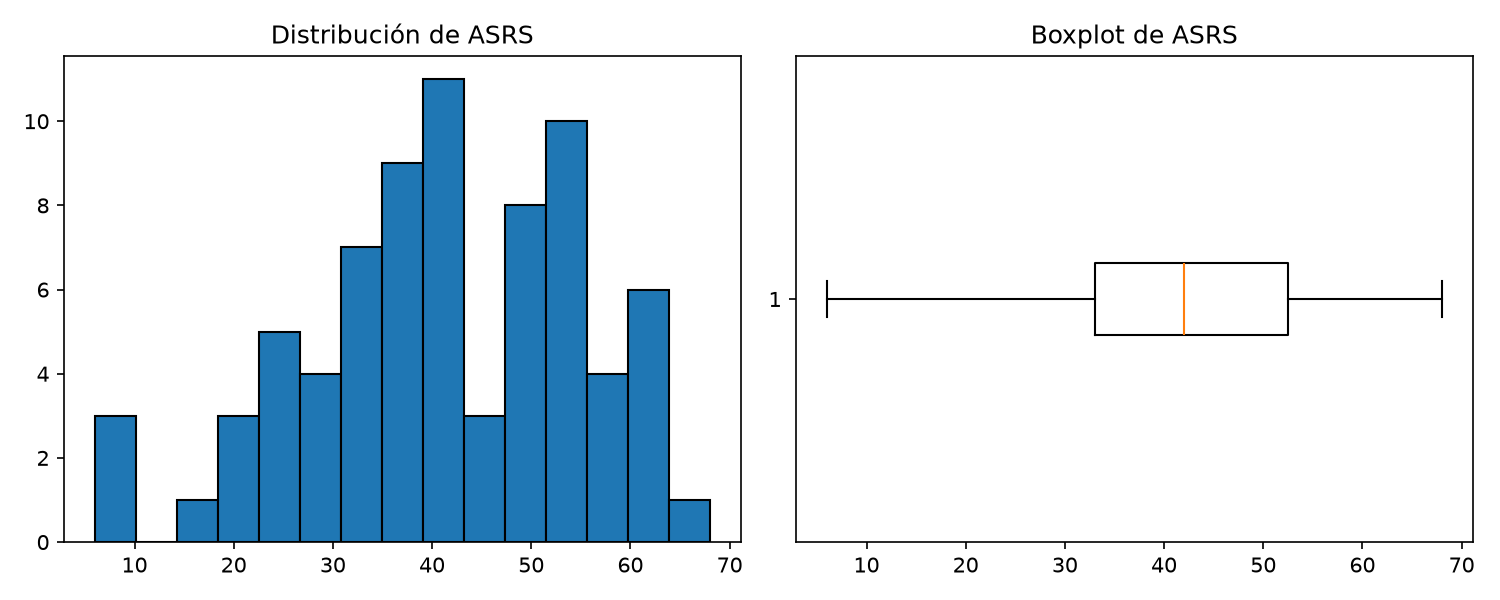
\includegraphics[width=0.88\textwidth]{../figures/asrs_distribucion.png}
  \caption{Histograma y diagrama de caja de la variable respuesta \texttt{ASRS} ($n = 75$).}
  \label{fig:asrs_dist}
\end{figure}

En la base integrada ($n = 75$), los puntajes de \texttt{ASRS} oscilan entre \textbf{6 y 68 puntos}, con media $= 41.39$, mediana $= 42.0$ y desviación estándar $= 13.90$ (Figura~\ref{fig:asrs_dist}). La distribución es aproximadamente simétrica, con una ligera cola izquierda formada por tres pacientes con puntajes bajos (entre 6 y 10). El diagrama de caja no muestra valores atípicos y la cercanía entre media y mediana indica ausencia de sesgo fuerte que obligue a transformar $Y$ de entrada.

\subsection{Coeficientes de correlación de Pearson ($r$) (Rúbrica 1b)}

Se calculó la correlación de Pearson ($r$) y su $p$-valor frente a \texttt{ASRS} para las variables numéricas candidatas (Tabla~\ref{tab:corr}). Dado que las variantes \textit{Adhd}, \textit{General} y \textit{Neuro} del CPT-II corresponden a la misma métrica contrastada contra distintos baremos de referencia, se adoptó consistentemente la versión \textit{General}.

\begin{table}[H]
  \centering
  \caption{Principales correlaciones de Pearson ($r$) respecto a \texttt{ASRS}.}
  \label{tab:corr}
  \small
  \begin{tabular}{l r r r l}
    \toprule
    \textbf{Variable candidata} & \textbf{$r$ con \texttt{ASRS}} & \textbf{$p$-valor} & \textbf{$n$} & \textbf{Interpretación} \\
    \midrule
    \texttt{WURS} & $0.685$ & $< 0.001$ & 74 & Positiva fuerte, altamente significativa \\
    \texttt{General TScore Commissions} & $0.526$ & $< 0.001$ & 75 & Positiva moderada, altamente significativa \\
    \texttt{General TScore DPrime} & $0.398$ & $< 0.001$ & 75 & Positiva moderada, significativa \\
    \texttt{HADS\_A} & $0.304$ & $0.011$ & 69 & Positiva débil a moderada, significativa \\
    \texttt{General TScore Omissions} & $0.287$ & $0.013$ & 75 & Positiva débil (inflada por un punto influyente) \\
    \texttt{MADRS} & $0.171$ & $0.154$ & 71 & No significativa \\
    \texttt{HADS\_D} & $0.112$ & $0.361$ & 69 & No significativa \\
    \texttt{AGE} & $-0.116$ & $0.320$ & 75 & No significativa \\
    \bottomrule
  \end{tabular}
\end{table}

\texttt{WURS} presenta la asociación lineal más fuerte ($r = 0.685$), respaldando la continuidad evolutiva del TDAH desde la infancia hasta la adultez. \texttt{Commissions} ($r = 0.526$) conecta una prueba conductual objetiva con la severidad autorreportada, mientras que \texttt{HADS\_A} ($r = 0.304$) refleja la comorbilidad ansiosa. En contraste, la depresión (\texttt{MADRS}, \texttt{HADS\_D}) y la edad (\texttt{AGE}) no muestran relación lineal significativa con \texttt{ASRS}.

\subsection{Gráficas de dispersión (Rúbrica 1a)}

\begin{figure}[H]
  \centering
  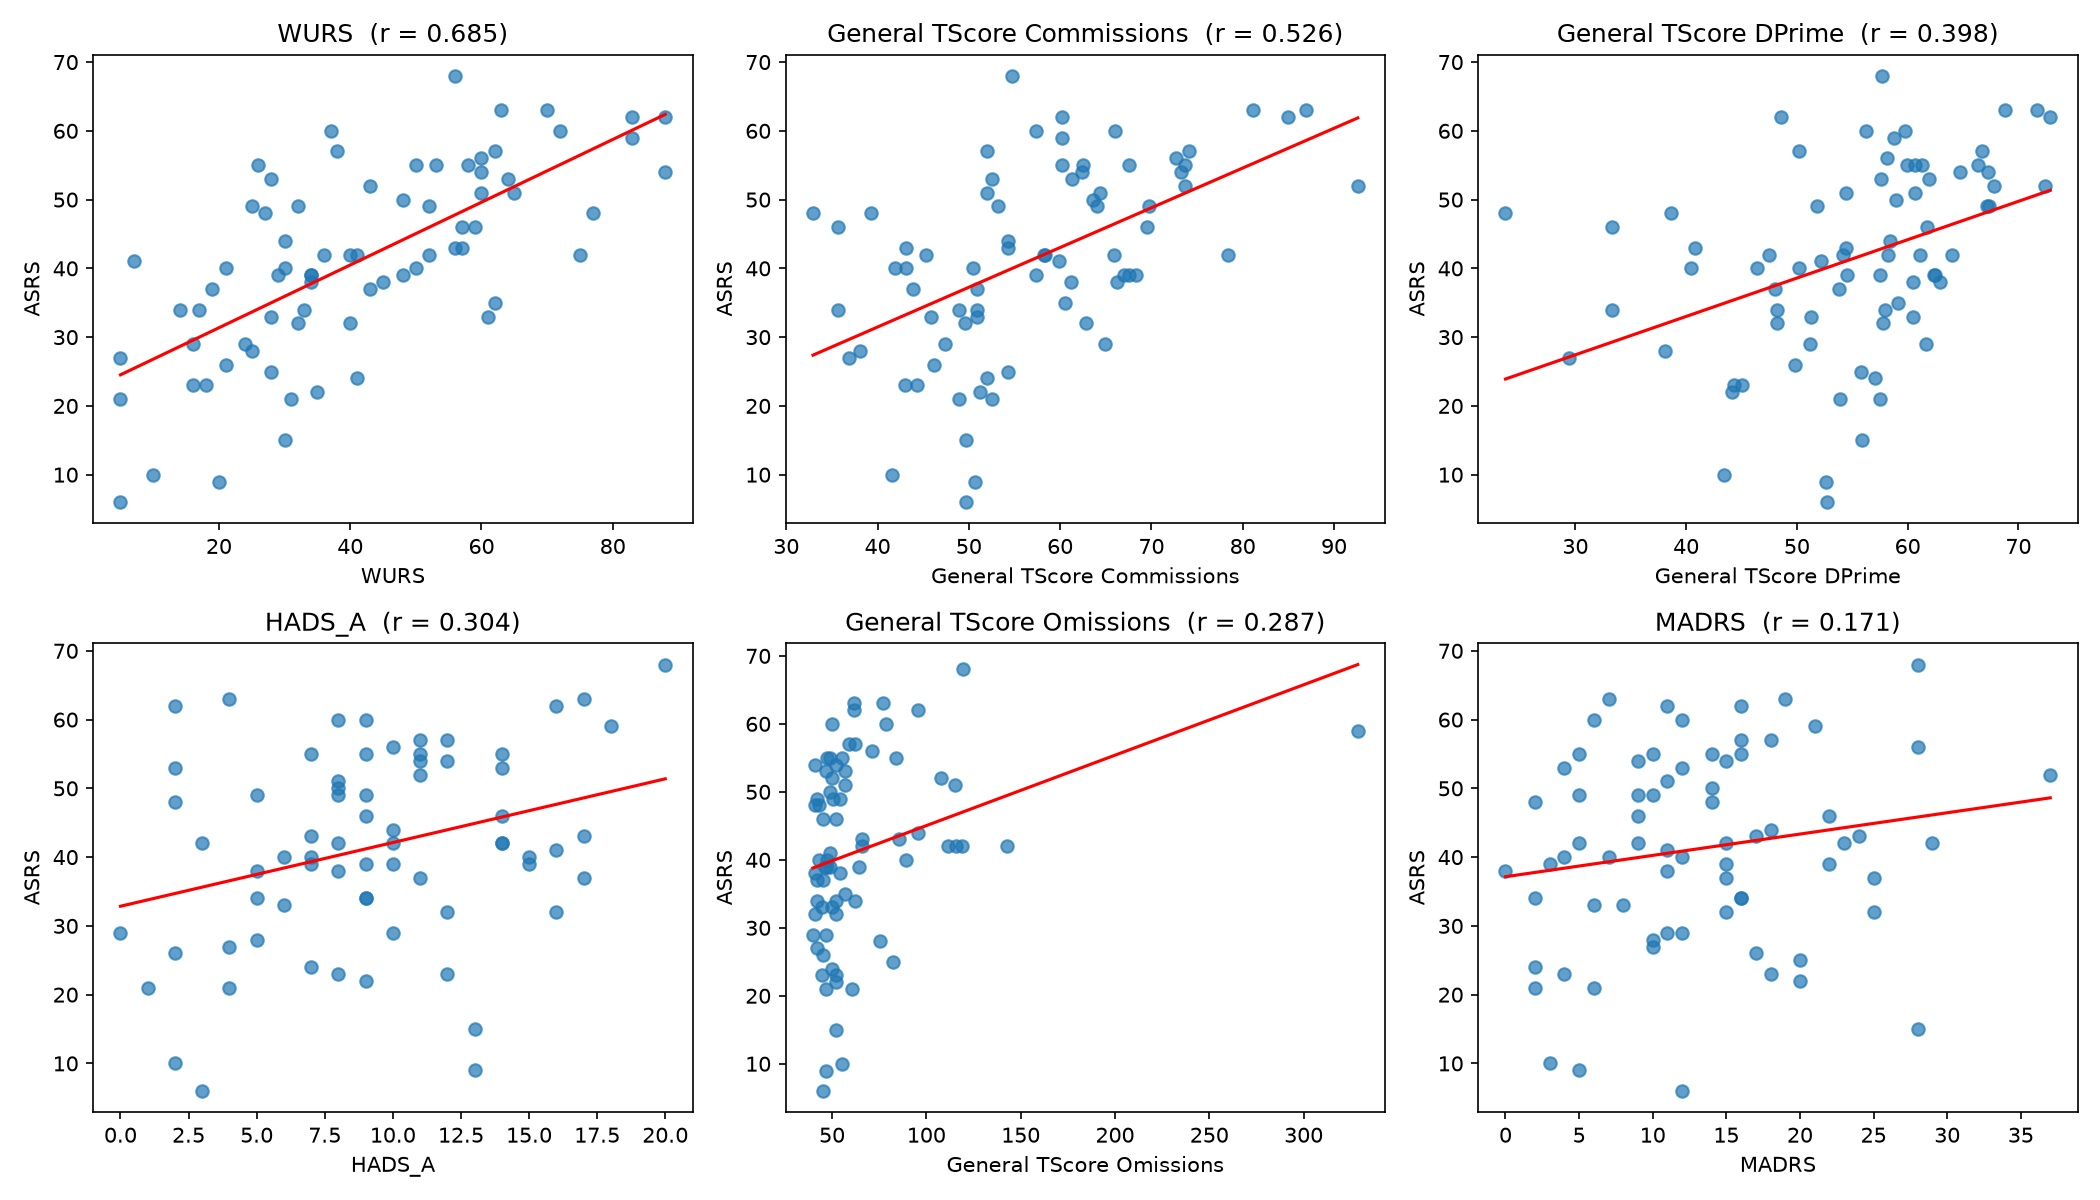
\includegraphics[width=0.95\textwidth]{../figures/dispersion_candidatas.png}
  \caption{Gráficas de dispersión con recta de tendencia para seis variables candidatas frente a \texttt{ASRS}.}
  \label{fig:scatter}
\end{figure}

El análisis visual (Figura~\ref{fig:scatter}) complementa al coeficiente $r$: \texttt{WURS} muestra una relación lineal positiva clara y dispersión homogénea; \texttt{Commissions} y \texttt{DPrime} muestran tendencia positiva con mayor dispersión; \texttt{HADS\_A} presenta pendiente leve y \texttt{MADRS} carece de tendencia. Destaca el caso de \texttt{Omissions}: la mayoría de los valores se agrupa entre 40 y 100, pero un único paciente cercano a 330 inclina la recta e infla artificialmente su $r = 0.287$, motivo por el cual se descartó.

\subsection{Selección final de predictores y validación de multicolinealidad (VIF)}

La matriz de correlación entre candidatas reveló colinealidad severa entre \texttt{General TScore Commissions} y \texttt{General TScore DPrime} ($r = 0.88$), por lo que se descartó \texttt{DPrime} y se conservó \texttt{Commissions} por su mayor correlación con \texttt{ASRS} y su interpretación directa como impulsividad. El resto de pares presentó $|r| \le 0.47$.

Para validar formalmente la ausencia de multicolinealidad se calculó el \textbf{Factor de Inflación de Varianza}:
\[
  \text{VIF}_j = \frac{1}{1 - R_j^2}
\]
donde $R_j^2$ es el coeficiente de determinación al regresar $X_j$ contra los demás predictores (con constante). Todos los valores quedaron muy por debajo del umbral $\text{VIF} < 5$ (Tabla~\ref{tab:vif}).

\begin{table}[H]
  \centering
  \caption{Factor de Inflación de Varianza (VIF) de los predictores confirmados ($n = 69$).}
  \label{tab:vif}
  \small
  \begin{tabular}{l r l}
    \toprule
    \textbf{Predictor ($X_j$)} & \textbf{VIF} & \textbf{Evaluación ($\text{VIF} < 5$)} \\
    \midrule
    \texttt{WURS} & $1.623$ & Cumple (sin multicolinealidad) \\
    \texttt{General TScore Commissions} & $1.390$ & Cumple (sin multicolinealidad) \\
    \texttt{HADS\_A} & $1.205$ & Cumple (sin multicolinealidad) \\
    \bottomrule
  \end{tabular}
\end{table}

% ==================== SECCIÓN 5 ====================
\section{Modelado por Mínimos Cuadrados Ordinarios (MCO) e interpretación}

\subsection{Planteamiento formal del modelo (Rúbrica 2a)}

El modelo poblacional en forma escalar es:
\[
  \text{ASRS}_i = \beta_0 + \beta_1\,\text{WURS}_i + \beta_2\,\text{Commissions}_i + \beta_3\,\text{HADS\_A}_i + \varepsilon_i, \qquad i = 1, \dots, 69
\]
bajo los supuestos clásicos de Gauss-Markov y normalidad: $\mathbb{E}[\varepsilon_i \mid \mathbf{X}] = 0$, $\text{Var}(\varepsilon_i \mid \mathbf{X}) = \sigma^2$, $\text{Cov}(\varepsilon_i, \varepsilon_j \mid \mathbf{X}) = 0$ ($i \neq j$) y $\varepsilon_i \sim \mathcal{N}(0, \sigma^2)$.

En notación matricial, $\mathbf{y} = \mathbf{X}\boldsymbol{\beta} + \boldsymbol{\varepsilon}$ con $\mathbf{y} \in \mathbb{R}^{69 \times 1}$ y $\mathbf{X} \in \mathbb{R}^{69 \times 4}$ (incluyendo la columna unitaria del intercepto). El estimador MCO que minimiza $S(\boldsymbol{\beta}) = (\mathbf{y} - \mathbf{X}\boldsymbol{\beta})^\top(\mathbf{y} - \mathbf{X}\boldsymbol{\beta})$ tiene solución cerrada:
\[
  \hat{\boldsymbol{\beta}} = (\mathbf{X}^\top \mathbf{X})^{-1}\mathbf{X}^\top \mathbf{y}
\]
La ecuación estimada resultante en \texttt{notebooks/03\_ols\_modeling\_and\_diagnostics.ipynb} es:
\[
  \widehat{\text{ASRS}}_i = 7.6350 + 0.3678\,\text{WURS}_i + 0.3079\,\text{Commissions}_i + 0.1273\,\text{HADS\_A}_i
\]

\subsection{Coeficientes, bondad de ajuste y pruebas $F$ y $t$ (Rúbrica 4a y 4b)}

\begin{table}[H]
  \centering
  \caption{Estimadores MCO, errores estándar, pruebas $t$ ($gl = 65$) e IC al 95\% ($n = 69$).}
  \label{tab:coef}
  \small
  \begin{tabular}{l r r r r c l}
    \toprule
    \textbf{Término} & $\hat{\beta}_j$ & \textbf{EE} & $t$ & $p$-valor & \textbf{IC 95\%} & \textbf{Significancia} \\
    \midrule
    \texttt{const} ($\hat{\beta}_0$) & $7.6350$ & $6.1095$ & $1.2497$ & $0.2159$ & $[-4.5666,\; 19.8365]$ & No significativo \\
    \texttt{WURS} ($\hat{\beta}_1$) & $0.3678$ & $0.0736$ & $4.9957$ & $< 0.0001$ & $[0.2208,\; 0.5149]$ & Significativo ($p < 0.001$) \\
    \texttt{Commissions} ($\hat{\beta}_2$) & $0.3079$ & $0.1162$ & $2.6507$ & $0.0101$ & $[0.0759,\; 0.5399]$ & Significativo ($p < 0.05$) \\
    \texttt{HADS\_A} ($\hat{\beta}_3$) & $0.1273$ & $0.2833$ & $0.4492$ & $0.6547$ & $[-0.4385,\; 0.6931]$ & No significativo \\
    \bottomrule
  \end{tabular}
\end{table}

\begin{itemize}
  \item \textbf{Bondad de ajuste (Rúbrica 4a):} $R^2 = 0.5341$ y $R^2_{\text{ajustado}} = 0.5126$, con $\text{RMSE} = 9.9015$ puntos en la escala \texttt{ASRS} ($\text{AIC} = 516.08$, $\text{BIC} = 525.02$). El modelo explica el \textbf{53.41\%} de la variabilidad total de \texttt{ASRS} (51.26\% ajustado por $k = 3$ predictores).
  \item \textbf{Prueba $F$ global (Rúbrica 4b):} para $H_0: \beta_1 = \beta_2 = \beta_3 = 0$, se obtiene $F(3, 65) = 24.8355$ con $p = 8.00 \times 10^{-11} < 0.001$, rechazando contundentemente $H_0$.
  \item \textbf{Pruebas $t$ individuales (Rúbrica 4b):} al nivel $\alpha = 0.05$, \texttt{WURS} ($t = 4.9957$) y \texttt{General TScore Commissions} ($t = 2.6507$) son significativos, mientras que \texttt{HADS\_A} ($t = 0.4492$) no lo es.
\end{itemize}

\subsection{Interpretación teórica y práctica de los parámetros (Rúbrica 2b)}

\begin{itemize}
  \item \textbf{Intercepto ($\hat{\beta}_0 = 7.6350$, $p = 0.2159$):} valor esperado de \texttt{ASRS} cuando todos los predictores valen cero. Carece de interpretación clínica porque $T = 0$ en \texttt{Commissions} se ubica a cinco desviaciones estándar bajo la media poblacional (mínimo observado $\approx 32.9$); su rol es estrictamente matemático.
  \item \textbf{\texttt{WURS} ($\hat{\beta}_1 = 0.3678$, $p < 0.0001$):} manteniendo constantes \texttt{Commissions} y \texttt{HADS\_A} (\textit{ceteris paribus}), cada punto adicional en síntomas infantiles aumenta la \texttt{ASRS} esperada en \textbf{0.3678 puntos} ($\approx 3.68$ puntos por cada 10 puntos de \texttt{WURS}).
  \item \textbf{\texttt{General TScore Commissions} ($\hat{\beta}_2 = 0.3079$, $p = 0.0101$):} \textit{ceteris paribus}, cada punto $T$ adicional en errores de comisión incrementa la \texttt{ASRS} esperada en \textbf{0.3079 puntos} ($\approx 3.08$ puntos por cada 10 puntos $T$). Confirma que una medida conductual objetiva aporta información independiente al autorreporte histórico.
  \item \textbf{\texttt{HADS\_A} ($\hat{\beta}_3 = 0.1273$, $p = 0.6547$):} su efecto es positivo pero no significativo (IC 95\% cruza el cero). Aunque correlacionaba bivariadamente con \texttt{ASRS} ($r = 0.304$), su efecto directo se diluye al controlar por \texttt{WURS} (con la cual comparte $r = 0.41$).
\end{itemize}

\textbf{Comparación del peso práctico (+1 desviación estándar muestral):} traduciendo cada coeficiente al cambio producido por una desviación estándar muestral ($n = 69$) se obtiene: \texttt{WURS} ($\text{DE} \approx 20.8 \Rightarrow +7.7$ puntos de \texttt{ASRS}), \texttt{Commissions} ($\text{DE} \approx 12.2 \Rightarrow +3.8$ puntos) y \texttt{HADS\_A} ($\text{DE} \approx 4.7 \Rightarrow +0.6$ puntos). La historia infantil pesa aproximadamente el doble que la impulsividad objetiva, mientras que la ansiedad prácticamente no aporta al controlar por ambas.

% ==================== SECCIÓN 6 ====================
\section{Evaluación visual y diagnóstico de supuestos}

\subsection{Valores reales frente a valores predichos (Rúbrica 4c)}

\begin{figure}[H]
  \centering
  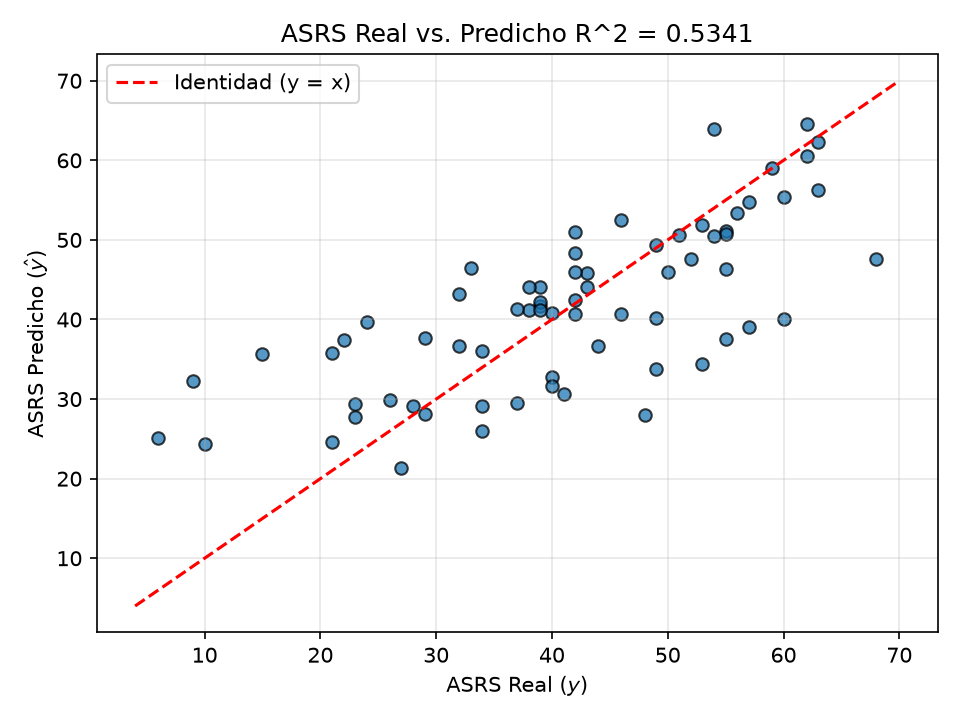
\includegraphics[width=0.62\textwidth]{../figures/ols_real_vs_predicho.png}
  \caption{Puntajes \texttt{ASRS} reales ($y$) frente a valores predichos ($\hat{y}$) con recta identidad ($y = x$).}
  \label{fig:real_pred}
\end{figure}

Los puntos se alinean de forma consistente en torno a la diagonal $y = x$ sin curvaturas sistemáticas (Figura~\ref{fig:real_pred}), reflejando $R^2 = 0.5341$ y la ligera regresión hacia la media en los extremos propia de MCO.

\subsection{Diagnóstico gráfico y formal de residuales}

\begin{figure}[H]
  \centering
  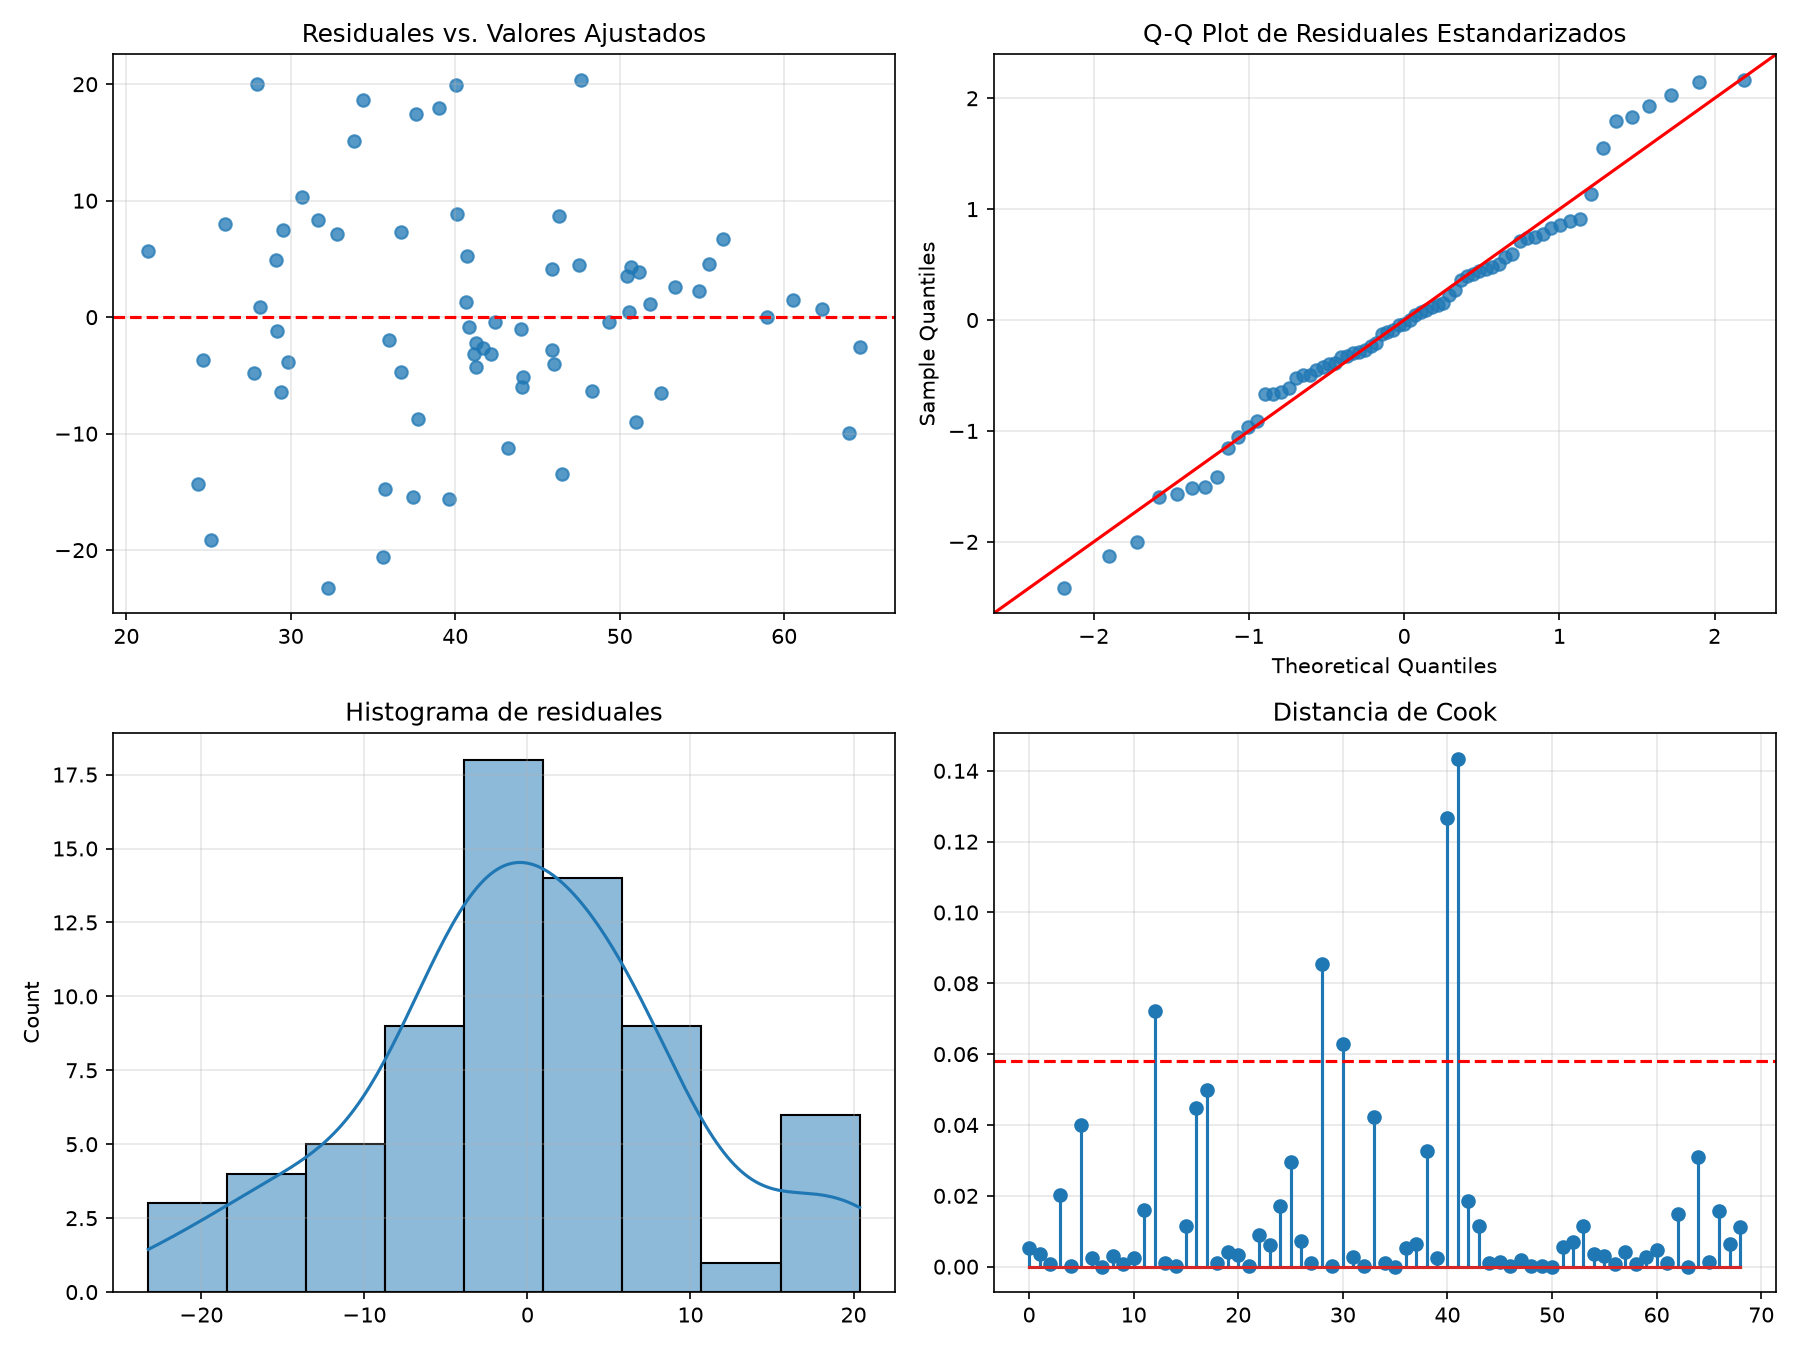
\includegraphics[width=0.92\textwidth]{../figures/ols_residual_diagnostics.png}
  \caption{Panel diagnóstico $2 \times 2$ de residuales del modelo MCO: residuales vs.\ ajustados, Q-Q plot, histograma y distancia de Cook.}
  \label{fig:resid}
\end{figure}

\begin{table}[H]
  \centering
  \caption{Pruebas estadísticas formales sobre los residuales del modelo MCO base ($n = 69$).}
  \label{tab:diag}
  \small
  \begin{tabular}{l l r r l}
    \toprule
    \textbf{Supuesto} & \textbf{Prueba / Métrica} & \textbf{Estadístico} & \textbf{$p$-valor / Umbral} & \textbf{Conclusión ($\alpha = 0.05$)} \\
    \midrule
    Normalidad & Shapiro-Wilk ($W$) & $0.9780$ & $p = 0.2634$ & \textbf{Cumple} (Omnibus $p = 0.885$, JB $p = 0.991$) \\
    Homocedasticidad & Breusch-Pagan ($\text{LM}$ / $F$) & $6.7705$ / $2.3573$ & $p = 0.0796$ / $0.0798$ & \textbf{Cumple al 5\%} (cercano al umbral) \\
    Independencia & Durbin-Watson ($\text{DW}$) & $2.174$ & Ref.\ $\approx 2.0$ & \textbf{Cumple} (sin autocorrelación) \\
    Puntos influyentes & Distancia de Cook ($D_i$) & 5 casos $> 4/n$ & \textbf{0 casos $> 1.0$} & \textbf{Estable} (sin observaciones patológicas) \\
    \bottomrule
  \end{tabular}
\end{table}

% ==================== SECCIÓN 7 ====================
\section{Evaluación de transformaciones y reversión a escala original (Rúbrica 3a)}

Dado que Breusch-Pagan arrojó un $p$-valor cercano al umbral ($p = 0.0796$) y \texttt{HADS\_A} resultó no significativa ($p = 0.6547$), en \texttt{notebooks/04\_transformations\_and\_forecasting.ipynb} se contrastaron tres alternativas frente al modelo base sobre los mismos $n = 69$ pacientes:

\begin{enumerate}
  \item \textbf{Log-Lineal ($\ln(\text{ASRS})$):} ajusta $\ln(Y_i) = \mathbf{x}_i^\top \boldsymbol{\gamma} + u_i$, con reversión insesgada a la escala original:
  \[
    \widehat{\text{ASRS}}_i = \exp\!\left(\widehat{\ln Y}_i + \frac{\hat{\sigma}_u^2}{2}\right)
  \]
  \item \textbf{Raíz cuadrada ($\sqrt{\text{ASRS}}$):} ajusta $\sqrt{Y_i} = \mathbf{x}_i^\top \boldsymbol{\delta} + v_i$, con reversión a la escala original:
  \[
    \widehat{\text{ASRS}}_i = \left(\widehat{\sqrt{Y}}_i\right)^2 + \hat{\sigma}_v^2
  \]
  \item \textbf{Parsimonioso (sin \texttt{HADS\_A}):} conserva únicamente \texttt{WURS} y \texttt{General TScore Commissions} ($k = 2$).
\end{enumerate}

\begin{table}[H]
  \centering
  \caption{Comparación de modelos candidatos en escala original de \texttt{ASRS} y supuestos ($n = 69$).}
  \label{tab:transf}
  \small
  \begin{tabular}{l c r r r r r}
    \toprule
    \textbf{Modelo} & $k$ & $R^2_{\text{adj}}$ (mod.) & $R^2$ (\texttt{ASRS}) & \textbf{RMSE (\texttt{ASRS})} & \textbf{Shapiro ($p$)} & \textbf{BP ($p$)} \\
    \midrule
    \textbf{Base lineal (3 pred.)} & 3 & $0.5126$ & $\mathbf{0.5341}$ & $\mathbf{9.6102}$ & $\mathbf{0.2634}$ & $\mathbf{0.0796}$ \\
    Log-Lineal $\ln(\text{ASRS})$ & 3 & $0.4030$ & $0.4427$ & $10.5101$ & $0.0000$ & $0.0268$ \\
    Raíz cuadrada $\sqrt{\text{ASRS}}$ & 3 & $0.4726$ & $0.5228$ & $9.7259$ & $0.0127$ & $0.0215$ \\
    Parsimonioso (sin \texttt{HADS\_A}) & 2 & $0.5185$ & $0.5326$ & $9.6251$ & $0.2829$ & $0.0411$ \\
    \bottomrule
  \end{tabular}
\end{table}

\textbf{Decisión y justificación:} Las transformaciones cóncavas ($\ln$ y $\sqrt{\cdot}$) están diseñadas para corregir colas derechas; como \texttt{ASRS} presenta una ligera \textbf{cola izquierda}, estiran el extremo inferior, \textbf{violan la normalidad} ($p < 0.0001$ y $p = 0.0127$), \textbf{empeoran la homocedasticidad} ($p = 0.0268$ y $p = 0.0215$) e \textbf{incrementan el RMSE} en escala original (Tabla~\ref{tab:transf}). Por su parte, eliminar \texttt{HADS\_A} sube marginalmente $R^2_{\text{adj}}$ ($0.5185$), pero \textbf{incumple homocedasticidad} al 5\% (Breusch-Pagan $p = 0.0411$). En consecuencia, se \textbf{conserva el modelo lineal base en escala original} al ser la única especificación que cumple simultáneamente todos los supuestos y minimiza el error en puntos \texttt{ASRS}.

% ==================== SECCIÓN 8 ====================
\section{Estimaciones puntuales y utilidad práctica (Rúbrica 5a)}

\subsection{Perfiles clínicos y pronósticos al 95\%}

Se definieron tres perfiles clínicos con los percentiles \textbf{P10, P50 y P90} de cada predictor en la muestra efectiva ($n = 69$, sin extrapolación). Con \texttt{.get\_prediction().summary\_frame(alpha=0.05)} se obtuvieron las estimaciones puntuales, el intervalo de confianza al 95\% de la media (IC 95\%) y el intervalo de predicción al 95\% individual (IP 95\%), incluyendo además el pronóstico revertido de $\sqrt{\text{ASRS}}$ como referencia (Tabla~\ref{tab:forecasts} y Figura~\ref{fig:forecasts}).

\begin{table}[H]
  \centering
  \caption{Estimaciones puntuales e intervalos al 95\% para tres perfiles clínicos ($n = 69$).}
  \label{tab:forecasts}
  \small
  \begin{tabular}{l r r r r c c r}
    \toprule
    \textbf{Perfil clínico} & \textbf{WURS} & \textbf{Comm.} & \textbf{HADS\_A} & $\widehat{\text{ASRS}}$ & \textbf{IC 95\% (media)} & \textbf{IP 95\% (indiv.)} & $\widehat{\text{ASRS}}_{\sqrt{Y}}$ \\
    \midrule
    Carga baja (P10) & 16 & 43 & 3 & $\mathbf{27.14}$ & $[22.48,\; 31.81]$ & $[6.82,\; 47.46]$ & $27.09$ \\
    Carga moderada (P50) & 38 & 57 & 9 & $\mathbf{40.31}$ & $[37.90,\; 42.72]$ & $[20.39,\; 60.23]$ & $39.54$ \\
    Carga alta (P90) & 65 & 73 & 16 & $\mathbf{56.06}$ & $[51.11,\; 61.00]$ & $[35.67,\; 76.44]^*$ & $57.62$ \\
    \bottomrule
    \multicolumn{8}{l}{\footnotesize $^*$El límite superior teórico de \texttt{ASRS} es 72, por lo que clínicamente el IP queda acotado a $[35.67,\; 72.00]$.}
  \end{tabular}
\end{table}

\begin{figure}[H]
  \centering
  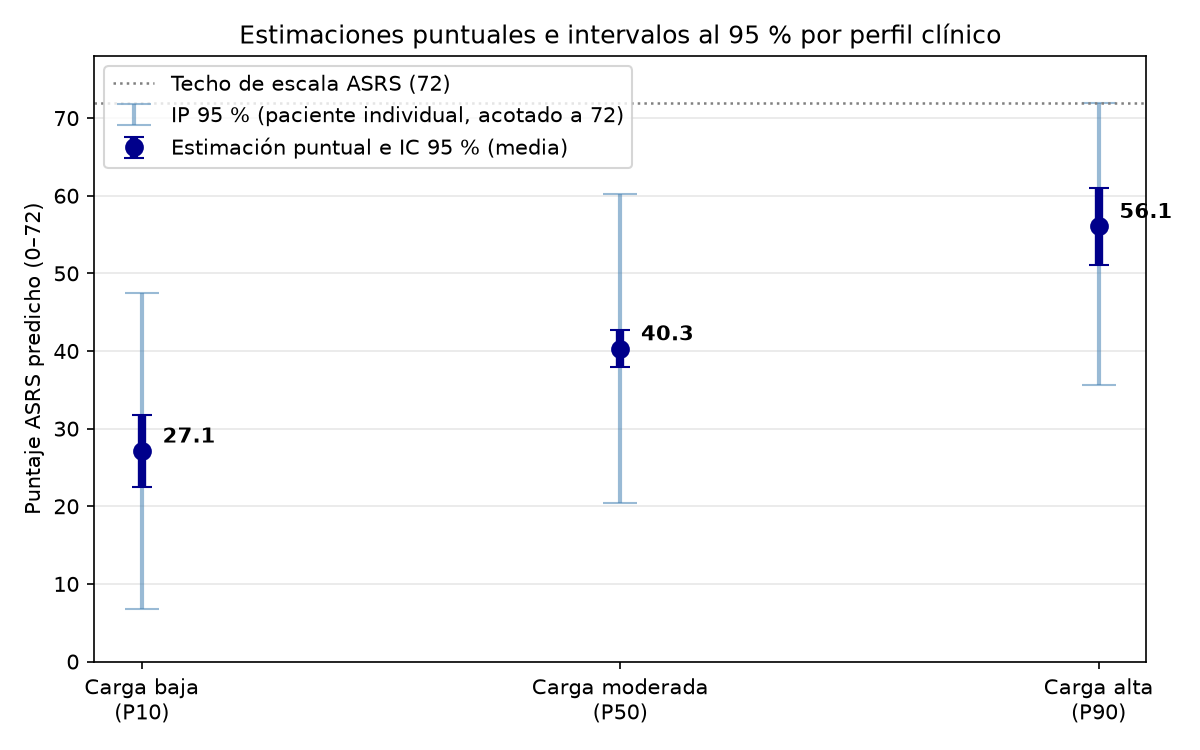
\includegraphics[width=0.78\textwidth]{../figures/ols_forecasts_profiles.png}
  \caption{Estimaciones puntuales, IC 95\% de la media e IP 95\% individual (acotado al techo de 72) por perfil clínico.}
  \label{fig:forecasts}
\end{figure}

\subsection{Utilidad clínica y limitaciones}

\textbf{Utilidad práctica:} El modelo separa con claridad perfiles de riesgo creciente ---una brecha de \textbf{28.92 puntos} entre carga baja y alta, con intervalos de confianza de la media completamente disjuntos---, lo que lo hace útil como herramienta cuantitativa de \textbf{apoyo al cribado y estratificación de riesgo} al combinar historia infantil (\texttt{WURS}) y desempeño objetivo (\texttt{CPT-II Commissions}).

\textbf{Limitaciones:} Para un paciente individual, el IP 95\% tiene una amplitud aproximada de $\pm 20$ puntos (reflejo de $\text{RMSE} = 9.90$ y de un $\approx 46.6\%$ de varianza no explicada). Sumado al tamaño muestral moderado ($n = 69$) y al carácter autorreportado de \texttt{ASRS} y \texttt{WURS}, el modelo \textbf{no sustituye una evaluación clínica diagnóstica integral}.

% ==================== SECCIÓN 9 ====================
\section{Conclusiones generales}

\begin{enumerate}
  \item Se construyó y validó un modelo de Regresión Lineal Múltiple por MCO ($n = 69$) libre de multicolinealidad ($\text{VIF} \le 1.623$) y de fuga de información que explica el \textbf{53.41\%} de la variabilidad de \texttt{ASRS} ($R^2_{\text{adj}} = 0.5126$, $F(3, 65) = 24.84$, $p < 0.001$).
  \item \texttt{WURS} ($\hat{\beta}_1 = 0.3678$, $p < 0.0001$) y \texttt{General TScore Commissions} ($\hat{\beta}_2 = 0.3079$, $p = 0.0101$) son predictores positivos y significativos, con \texttt{WURS} aportando aproximadamente el doble de impacto práctico por desviación estándar (+7.7 frente a +3.8 puntos). \texttt{HADS\_A} ($p = 0.6547$) pierde significancia directa al controlar por la historia infantil.
  \item El modelo lineal base en escala original satisface todos los supuestos clásicos (Shapiro-Wilk $p = 0.2634$, Breusch-Pagan $p = 0.0796$, Durbin-Watson $= 2.174$, 0 observaciones con Cook $> 1.0$) y supera en precisión y cumplimiento de supuestos a las transformaciones $\ln(\text{ASRS})$, $\sqrt{\text{ASRS}}$ (tras su reversión analítica) y al modelo parsimonioso sin \texttt{HADS\_A}.
  \item Los pronósticos sobre perfiles representativos (P10, P50 y P90) confirman la coherencia del modelo como herramienta de apoyo al cribado, delimitando con transparencia la incertidumbre a nivel individual.
\end{enumerate}

% ==================== REFERENCIAS ====================
\section*{Referencias}
\addcontentsline{toc}{section}{Referencias}

\begin{itemize}
  \item Conners, C. K. (2000). \textit{Conners' Continuous Performance Test II (CPT II)}. Multi-Health Systems.
  \item Hicks, S. A., Stautland, A., Fasmer, O. B., F\o{}rland, W., Hammer, H. L., Halvorsen, P., \ldots{} Riegler, M. A. (2021). HYPERAKTIV: An activity dataset from patients with attention-deficit/hyperactivity disorder (ADHD). \textit{Proceedings of the 12th ACM Multimedia Systems Conference}.
  \item Kessler, R. C., Adler, L., Ames, M., et al. (2005). The World Health Organization Adult ADHD Self-Report Scale (ASRS). \textit{Psychological Medicine}, 35(2), 245--256.
  \item Ward, M. F., Wender, P. H., \& Reimherr, F. W. (1993). The Wender Utah Rating Scale: An aid in the retrospective diagnosis of childhood attention deficit hyperactivity disorder. \textit{American Journal of Psychiatry}, 150(6), 885--890.
  \item Zigmond, A. S., \& Snaith, R. P. (1983). The Hospital Anxiety and Depression Scale. \textit{Acta Psychiatrica Scandinavica}, 67(6), 361--370.
\end{itemize}

\end{document}

